\definecolor{wsdred}{HTML}{8E1728}



\tikzset{every picture/.style={line width=0.75pt}} %set default line width to 0.75pt        

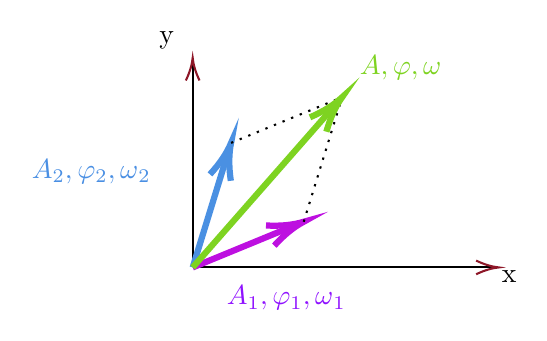
\begin{tikzpicture}[x=0.75pt,y=0.75pt,yscale=-1,xscale=1]
%uncomment if require: \path (0,15225); %set diagram left start at 0, and has height of 15225

%Straight Lines [id:da5927370156317948] 
\draw    (146,906) -- (291.5,906) ;
\draw [shift={(293.5,906)}, rotate = 180] [color={wsdred}  ][line width=0.75]    (10.93,-3.29) .. controls (6.95,-1.4) and (3.31,-0.3) .. (0,0) .. controls (3.31,0.3) and (6.95,1.4) .. (10.93,3.29)   ;
%Straight Lines [id:da34962116656860287] 
\draw [color={rgb, 255:red, 189; green, 16; blue, 224 }  ,draw opacity=1 ][line width=2.25]    (146,906) -- (195.8,885.52) ;
\draw [shift={(199.5,884)}, rotate = 157.65] [color={rgb, 255:red, 189; green, 16; blue, 224 }  ,draw opacity=1 ][line width=2.25]    (17.49,-5.26) .. controls (11.12,-2.23) and (5.29,-0.48) .. (0,0) .. controls (5.29,0.48) and (11.12,2.23) .. (17.49,5.26)   ;
%Straight Lines [id:da8962545520745455] 
\draw    (146,906) -- (146,807) ;
\draw [shift={(146,805)}, rotate = 90] [color={wsdred}  ][line width=0.75]    (10.93,-3.29) .. controls (6.95,-1.4) and (3.31,-0.3) .. (0,0) .. controls (3.31,0.3) and (6.95,1.4) .. (10.93,3.29)   ;
%Straight Lines [id:da9101145846792975] 
\draw [color={rgb, 255:red, 74; green, 144; blue, 226 }  ,draw opacity=1 ][line width=2.25]    (146,906) -- (163.32,849.82) ;
\draw [shift={(164.5,846)}, rotate = 107.14] [color={rgb, 255:red, 74; green, 144; blue, 226 }  ,draw opacity=1 ][line width=2.25]    (17.49,-5.26) .. controls (11.12,-2.23) and (5.29,-0.48) .. (0,0) .. controls (5.29,0.48) and (11.12,2.23) .. (17.49,5.26)   ;
%Straight Lines [id:da7014505903865442] 
\draw [color={rgb, 255:red, 0; green, 0; blue, 0 }  ,draw opacity=1 ][line width=0.75]  [dash pattern={on 0.84pt off 2.51pt}]  (199.5,884) -- (218,824) ;
%Straight Lines [id:da16436515246039618] 
\draw [color={rgb, 255:red, 0; green, 0; blue, 0 }  ,draw opacity=1 ][line width=0.75]  [dash pattern={on 0.84pt off 2.51pt}]  (164.5,846) -- (218,824) ;
%Straight Lines [id:da04823563439608747] 
\draw [color={rgb, 255:red, 126; green, 211; blue, 33 }  ,draw opacity=1 ][line width=2.25]    (146,906) -- (215.36,827.01) ;
\draw [shift={(218,824)}, rotate = 131.28] [color={rgb, 255:red, 126; green, 211; blue, 33 }  ,draw opacity=1 ][line width=2.25]    (17.49,-5.26) .. controls (11.12,-2.23) and (5.29,-0.48) .. (0,0) .. controls (5.29,0.48) and (11.12,2.23) .. (17.49,5.26)   ;

% Text Node
\draw (293.5,906) node [anchor=north west][inner sep=0.75pt]   [align=left] {x};
% Text Node
\draw (129,863) node [anchor=north west][inner sep=0.75pt]   [align=left] {};
% Text Node
\draw (128.5,791) node [anchor=north west][inner sep=0.75pt]   [align=left] {y};
% Text Node
\draw (67,852.5) node [anchor=north west][inner sep=0.75pt]    {$\textcolor[rgb]{0.29,0.56,0.89}{A}\textcolor[rgb]{0.29,0.56,0.89}{_{2}}\textcolor[rgb]{0.29,0.56,0.89}{,\varphi }\textcolor[rgb]{0.29,0.56,0.89}{_{2}}\textcolor[rgb]{0.29,0.56,0.89}{,\omega }\textcolor[rgb]{0.29,0.56,0.89}{_{2}}\textcolor[rgb]{0.29,0.56,0.89}{\ }$};
% Text Node
\draw (161,913.5) node [anchor=north west][inner sep=0.75pt]    {$\textcolor[rgb]{0.56,0.07,1}{A}\textcolor[rgb]{0.56,0.07,1}{_{1}}\textcolor[rgb]{0.56,0.07,1}{,\varphi }\textcolor[rgb]{0.56,0.07,1}{_{1}}\textcolor[rgb]{0.56,0.07,1}{,\omega }\textcolor[rgb]{0.56,0.07,1}{_{1}}$};
% Text Node
\draw (225,802.5) node [anchor=north west][inner sep=0.75pt]  [color={rgb, 255:red, 126; green, 211; blue, 33 }  ,opacity=1 ]  {$A,\varphi ,\omega $};

\end{tikzpicture}